\documentclass[conference]{IEEEtran}
\usepackage{cite}
\usepackage{amsmath,amssymb,amsfonts}
\usepackage{algorithmic}
\usepackage{graphicx}
\usepackage{textcomp}
\usepackage{xcolor}
\def\BibTeX{{\rm B\kern-.05em{\sc i\kern-.025em b}\kern-.08em
    T\kern-.1667em\lower.7ex\hbox{E}\kern-.125emX}}
\begin{document}

\title{Emotion analysis in dataset}


\author{\IEEEauthorblockN{Meriem Aggoune}
\IEEEauthorblockA{\textit{dept. name of organization (of Aff.)} \\
\textit{name of organization (of Aff.)}\\
City, Country \\
email address or ORCID}
\and
\IEEEauthorblockN{ Lauri Heikka}
\IEEEauthorblockA{\textit{Faculty of Information Technology and Electrical Engineering} \\
\textit{Univ. of Oulu}\\
Oulu, Finland \\
lauri.heikka@student.oulu.fi}
\and
\IEEEauthorblockN{Anusha Ihalapathiranae}
\IEEEauthorblockA{\centerline{Faculty of Information Technology and Electrical Engineering} \\
\textit{Univ. of Oulu}\\
Oulu, Finland \\
anusha.ihalapathirana@student.oulu.fi}

}

\maketitle

\begin{abstract}
We document a series of experiments on using a variety of natural language processing methods to classify emotions conveyed by sentences. In particular, we compare word categorizations, semantic similarity approaches and machine learning approaches. The machine learning approaches consist of classification models based on bag-of-words representations and convolutional neural networks applied on word embeddings. Our results indicate that machine learning approaches outperform string matching and semantic similarity with a considerable margin. Within the machine learning approaches, convolutional neural networks with word embeddings provide an improvement in accuracy of around 3-5 percentage points over bag-of-words models. The best accuracy on a hold-out validation set, around 93\%, is achieved with a CNN approach using pre-trained word2vec embeddings. However, custom-trained word embeddings provide similar performance with less computational overhead.
\end{abstract}

\begin{IEEEkeywords}
natural language processing, text classification, sentiment analysis
\end{IEEEkeywords}

\section{Group info}
Group 10

Members: Meriem Aggoune, Lauri Heikka, Anusha Ihalapathiranae

Title: Emotion Analysis in Dataset

Github: https://github.com/MeriemLil/NLP\_Project

\section{Introduction}
Emotions are feelings that caused by a situation person interact with. It is also associate with person’s character, mood, personality and motivation. People express their feelings and emotions using verbally and non-verbally such as words, intonation of voice, facial expressions, gestures, and tears. Nowadays people tend to communicate their ideas, opinions, and feelings through social medias, Such as tweeter, facebook, instergram. People filled with lot emotions and they commonly use written text to express their emotions and feelings through social medias. Categorizing text into emotion types is known as emotion analysis. Sentiment analysis detect positive, negative, and neutral feelings from text and emotion analysis detect the types of feelings, emotion state, in the text \cite{emotiondetection}.

Emotion analysis takes major role in some applications which use emotion recognition, and it is a growing research area. There are supervised and unsupervised approaches can be found in this research area. A novel unsupervised context-based approach represents in \cite{unsupervisedemotiondetection} to detect emotions from text in sentence level. Their approached does not need any existing manually created lexicons and they used semantic relation between words and emotion type. They fine tune scores using syntactic dependencies within the sentence structure and proves this model provide more accurate results than other unsupervised approaches. Research carried out in \cite{jan2020emotion} paid their attention towards capturing semantic features in the text. Authors used distributional semantic model to calculate the semantic relatedness of the emotion in the text and they achieved accuracy of 71.79\% without training or annotation of data use.

A lot of research had been carried out on sentiment analysis and emotion analysis problem in many different languages. Bag-of-words representations, first suggested by Luhn in the 1950s \cite{luhn}, are an important advance, and still a commonly applied tool for natural language processing tasks like text classification. In these models, text is represented as a sparse feature matrix, where features represents the occurrences of a given word in a text. Earlier approaches involved counting the occurrences of words. Later, improvements have been suggested that offset the number of occurrences of a word in a given text by the frequency of the word's occurrence in other texts in the corpus \cite{tfidf}. The most notable of these approaches is the term frequency–inverse document frequency (tf-idf) weighting.

In a seminal, of applying machine learning algorithms using a bag-of-words representation \cite{joachims-svm} propose the use of support vector regressions with the tf-idf matrix approach. Using this approach, they achieve notable improvements over the state-of-the-art benchmarks at the time. In a more recent example, \cite{chaffaretal}  demonstrate their work on supervised machine learning approach to recognize the emotion types using emotion annotated dataset which combined news headlines, fairy tales and blogs. They use bag of words and N-grams and proved that support vector machines classifier shows better performance and generalization than the other classifiers they used. 

\cite{kim-2014-convolutional} introduce convolutional neural networkds for text categorization. Similar concepts are explored by e.g. \cite{johnsonetal}, with a low complexity word level deep convolutional neural network for text categorization. \cite{dossantosetal} propose a new convolutional neural network that exploits from character to sentence level information to perform sentiment analysis of short texts. They found that combining small text with prior knowledge is effective.

Research in \cite{bert} introduce a new language representation model, BERT, a pretrained deep bidirectional representations from unlabeled text. They used conditioning on both information before and after a given word in all layers.BERT and successors inspired by it (see e.g. \cite{xlnet}), have massively improved the state-of-the-art in many language understandings tasks. For text classification, \cite{ bertclassification} used BERT provide general solution for BERT fine tuning in a text classification setting. Similarly, research on \cite{xu2020improving} improves the fine tuning of BERT using two effective mechanisms: self-ensemble and self-distillation.

In this research we are focusing on emotion analysis using word categorizations, semantic similarity approaches and machine learning approaches.
\section{Data and Methodologies}
\subsection{Datasets and sources}
Our main dataset of interest is a labeled dataset of 20 000 sentences with between 3 and 66 words. The dataset is provided by \cite{kaggledata}. The sentences are labeled to convey one of six different emotions: fear, anger, joy, love, surprise and sadness. The dataset is collected following the approach of \cite{saravia-etal-2018-carer}. The sentences are tweets, and the emotion labels are hashtags at the end of the tweet. The sentences are preprocessed in that they contain no punctuation or special characters and all words are lowercase.

The dataset has a predefined split into training, test and validation samples, with 16 000, 2 000 and 2 000, respectively. Because the semantic similarity and string matching approaches do not employ any predictive modeling, in these sections we use the all 20 000 sentences to measure prediction accuracy. For the machine learning approaches, we use the training set for model training, the test set for model selection and hyperparameter tuning, and reserve the validation dataset as a final benchmark, to ensure a fair comparison accross approaches.

In addition, we use pre-trained, 300-dimensional word2vec embeddings  from \cite{mikolov2013distributed} and pre-trained fastText embeddings from \cite{bojanowski2016enriching}. Both datasets consist of 300-dimensional word embeddings, with embeddings for 3 and 1 million english words, respectively. For the string matching, we use the Harvard General Inquirer dataset, which contains categorizations for around 11 000 english words.

\subsection{Harvard Inquirer and String Matching}
The first method we explore is to categorize each word in Harvard General Inquirer \cite{harvardgeneralinquirer} to each emotion type. We use a filtering technique to this categorization. To identify words related to love emotion, we include Harvard General Inquirer words with that are labeled Affil label and exclude words associated with Negative label. The categories used for all six labels is reported in Table~\ref{taba3}. We store this information into a database and then compute the occurrences of words associated with each label for each sentence and predict the label of a sentence to be the category with the highest number of words.

\subsection{Empath Client Categories}
The next method we explore is to use the Empath Client \cite{empathclient}, a text analyzing tool with a pre-buildt category set. We identify categories related to each sentence using the Empath client. Then for all the identified categories, we compute empath category similarity with each label using the concept of lowest common hypernymy. We then associate each category provided by the Empath client with the emotion that has the highest similarity. Then, we use the label assigned to each category of a sentence to identify the label that has the highest number of occurrences. The emotion is predicted to be this label. The empath client categorization has a category for each of our labels as well, so we also experiment using only the exact emotion category.
\subsection{Semantic Similarity}
asd
\subsection{SentiStrength Sentiment Scores}
As part of the project specification, we also use the SentiStrength client \cite{sentistrength}, to compute sentiment scores. These can be potentially be used as an additional feature in any approach to distinguish between the negative and positive emotions. However, intuitively, the more difficult task is distinguishing between different positive emotions and between different negative emotions. For this purpose, the sentiment scores are unlikely to provide added benefit. Considering this, and the fact that the simple approaches perform quite poorly, we do not explore the effects of these sentiment scores onto the accuracy of different models. Sentiment scores are still delivered as part of the project database, as suggested in the project specification.

\subsection{Bag-of-Words Models}

\subsection{Convolutional Neural Networks}

\subsubsection{Model architecture}

We replicate the convolutional neural network architecture used in \cite{kim-2014-convolutional}. The architecture is outlined in fig.~\ref{fig1}. Sentences are represented as $n\times k$ matrices of word vector embeddings, where \emph{n} refers to the length of the sentences and $k$ to the dimension of the word vectors.

\begin{figure*}[htbp]
\centerline{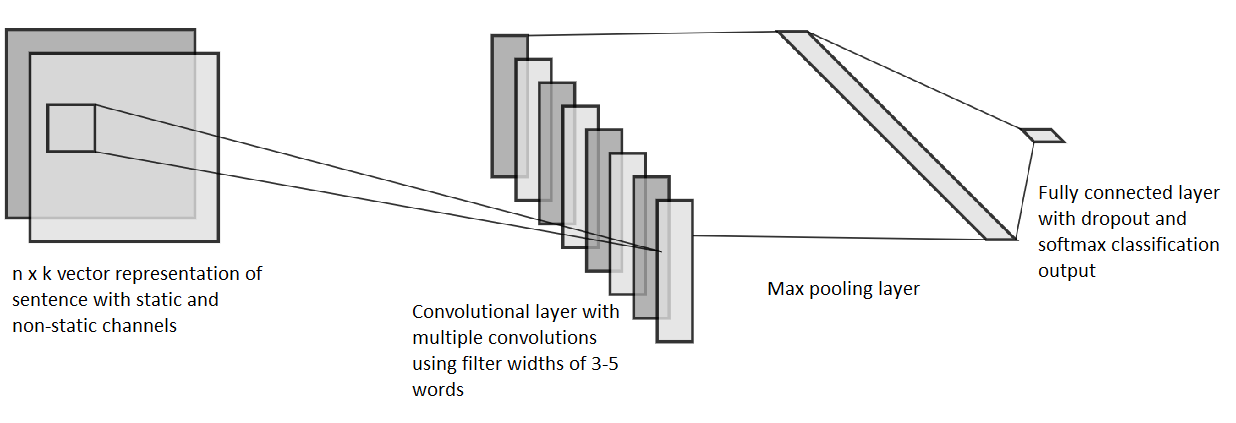
\includegraphics[width = \textwidth]{fig1.png}}
\caption{CNN model architecture}
\label{fig1}
\end{figure*}

All sentences are zero-padded to length $n$.
\footnote{A similar architecture is proposed in \cite{johnsonetal}, but one where sentences are not padded to a fixed length.  Note that, the application of max-pooling is likely to make the zero-padding inconsequential.}
Then a set of 1-dimensional convolutions are applied on the sentences. For each sentence, a feature $c_i$ is generated by the convolution
\begin{equation}
c_i = f(w * x_{i:i+h-1} + b)\label{eq1}
\end{equation}
where $h$ refers to the length of the convolution window, $w$ are the filter weights of the convolution operation, $b$ is an added bias term, and $f$ is a non-linear activation function. A feature map $c$ is then an $n-h+1$-dimensional vector of these features.

Equation \eqref{eq1} describes only one feature map produced by one convolution filter, while the model can consist of an arbitrary number of these feature maps. Then, for each feature map, max-pooling is applied, such that the largest feature value $c_{i-max}$ is selected. This operation produces a vector of final features with dimension equal to the number of feature maps used. These features are then connected to the final, 6-dimensional softmax output with a fully connected layer.

For regularization the original paper uses dropout on the penultimate layer. Dropout is a commonly used regularization method in neural networks. It hides each of the final features from the output layer with some probability $p$, preventing the co-adaptation of the different features. In addition, we experiment with another common method of avoiding overfitting; an $l_2$-norm regularization across the layer weights. The $l_2$ regularization penalizes large weight vectors, preventing overfitting.  Finally, following \cite{kim-2014-convolutional}, we also constrain the $l_2$ - norms of the weight vectors $w$ to be a maximum of a fixed size $s$. Note that the norm-constraint is most often applied to prevent an exploding gradients problem rather than to prevent overfitting.

Something on the different modes of the model.....


\subsubsection{Word Embeddings}
The purpose of using word embeddings in the CNN model is to provide a $k$ dimensional numerical representation that can be input to the neural network. The general idea of these embedding model is to identify useful word embeddings by training a shallow neural network on a word prediction task using a large text corpus. Model training positions word vectors in the $k$-dimensional vector space such that similarities between word vector embeddings represent the semantic similarity between the words.

In \cite{kim-2014-convolutional}, pre-trained Word2Vec embeddings from \cite{mikolov2013distributed, mikolov2013efficient} are used. In addition to replicating this approach, we consider a few alternatives. First, we test pretrained fastText embeddings from \cite{bojanowski2016enriching, joulin2016bag}. Second, we explore explore training our own word2vec and fastText embeddings using the papers cited above.

 \cite{mikolov2013efficient} apply two approaches to training a word2vec model, a continuous bag-of-words (CBOW) model and a continuous skip-gram model. The idea for the CBOW model  is to train a shallow neural network to predict a current word in a sentence given a pre-specified window of words around it. The skip-gram model instead predicts the words around a given word wihin a pre-specified range in the sentence. The pre-trained word2vec vectors that we use in the experiments are trained using the skip-gram architecture. For our custom-trained embeddings, we instead use the CBOW model to provide a comparison.

FastText \cite{bojanowski2016enriching} is proposed as an extension to the word2vec model. The fastText model introduces subword information, in the form of character $n$-grams, by representing words as the sum of the vector representations of its $n$-grams. This means that or example if $n = 3$, then the word $what$ is represented by: $<wh, wha, hat, he>$ $n$-grams and the sequence $<what>$ itself. The authors in \cite{bojanowski2016enriching} argue that this allows to incorporate the internal structure of words and to produce more reliable representations for rare words.


\subsubsection{Hyperparameters and training}
 For the custom-trained word2vec and fastText models, we use a maximum distance between predicted words of five and early stopping on a generic word analogy evaluation task. Since this is a secondary objective, we do not explore alternative setups or model tuning for the word embedding task, and focus on tuning the CNN instead. As for the dimension of the word embeddings, we experiment with 50-, 100- and 300-dimensional word embeddings for the custom-trained word embeddings. With the pre-trained embeddings, we are restricted to the commonly available 300-dimensional word embeddings.

For all CNN models, we use sentence length $n = 70$ and convolution windows $h$ of 3, 4 and 5.  following the original paper. We use a rectified linear unit (ReLU) activation function for the convolutions, and a softmax activation for the output layer. The original paper uses Adadelta \cite{adadelta} optimization, but we achieve faster convergence with an Adam \cite{adam} update rule. We train using mini-batches of 50 sentences, a learning rate of $10^{-3}$ and the cross-entropy loss function. We also employ early stopping based on the models cross-entropy loss on the test dataset.

For the input mode, we introduce. The full set and ranges of the hyperparameters that we tune is reported in able~\ref{tabahp}. The original paper uses a set of 100 convolutions. We treat the number of convolutions as a hypermeter, and experiment with from 50 to 250 convolutions. Note that the number of convolutions is applied for each of the three window lengths resulting in a total of $3 * number of feature maps$ convolutions. We explore 

\section{Results and Discussion}

\subsection{Word categorizations and semantic similarity}

\begin{table}[htbp]
\caption{Word categorizations and semantic similarity accuracies}
\begin{center}
\begin{tabular}{|c|c|}
\hline
\textbf{Classifier}&\multicolumn{1}{|c|}{\textbf{Accuracy}} \\ 

\hline
Harvard String Matching & 0.336 \\ 
\hline
Empath Client & 0.160 \\ 
\hline
Empath Client with exact categories & 0.183 \\ 
\hline
Semantic Similarity - One synset & 0.269 \\ 
\hline
Semantic Similarity - All synset & 0.240 \\ 
\hline
\end{tabular}
\label{tab1}
\end{center}
\end{table}

\subsection{Model selection for bag-of-words}
Table~\ref{tab5} reports the accuracies on the test dataset used for model selection.
\begin{table}[htbp]
\caption{Maximum accuracy on the test dataset across different bag-of-words setups}
\begin{center}
\begin{tabular}{|c|c|c|}
\hline
\textbf{}&\multicolumn{2}{|c|}{\textbf{}} \\ 
\cline{2-3}
\textbf{parameter} & \textbf{\textit{value}}& \textbf{\textit{score}} \\ 
\hline
vectorizer & CountVectorizer & 0.886 \\ 
\cline{2-3}
 & TfidfVectorizer & 0.888 \\ 
\hline
stopwords & nltk & 0.888 \\ 
\cline{2-3}
 & none & 0.878 \\ 
\cline{2-3}
 & sk & 0.884 \\ 
\hline
lemmatize & 0 & 0.888 \\ 
\cline{2-3}
 & 1 & 0.886 \\ 
\hline
max features  & 100 & 0.396 \\ 
\cline{2-3}
  & 500 & 0.728 \\ 
\cline{2-3}
 & 1000 & 0.865 \\ 
\cline{2-3}
  & 2000 & 0.880 \\ 
\cline{2-3}
  & 3000 & 0.886 \\ 
\hline
classifier & DecisionTreeClassifier & 0.866 \\ 
\cline{2-3}
 & GradientBoostingClassifier & 0.849 \\ 
\cline{2-3}
 & LogisticRegression & 0.878 \\ 
\cline{2-3}
 & MultinomialNB & 0.859 \\ 
\cline{2-3}
 & RandomForestClassifier & 0.888 \\ 
\cline{2-3}
 & SVC & 0.876 \\ 
\hline
\end{tabular}
\label{tab5}
\end{center}
\end{table}

\subsection{Validation set performance of best models}
Table~\ref{tab1} reports the accuracies on the test dataset used for model selection.

\begin{table}[htbp]
\caption{Validation and test set accuracies for best models}
\begin{center}
\begin{tabular}{|c|c|c|}
\hline
\textbf{}&\multicolumn{2}{|c|}{\textbf{Accuracy}} \\ 
\cline{2-3}
\textbf{Classifier} & \textbf{\textit{Validation}}& \textbf{\textit{Test}} \\ 
\hline
MultinomialNB & 0.681 & 0.694 \\ 
\hline
LogisticRegression & 0.872 & 0.864 \\ 
\hline
RandomForestClassifier & 0.899 & 0.89 \\ 
\hline
CNN fastText pretrained & 0.925 & 0.928 \\ 
\hline
CNN Word2Vec own & 0.928 & 0.929 \\ 
\hline
CNN fastText own & 0.928 & 0.931 \\ 
\hline
CNN Word2Vec pretrained & 0.930 & 0.928 \\ 
\hline
\end{tabular}
\label{tab1}
\end{center}
\end{table}

\begin{table}[htbp]
\caption{Validation precision and recall for best models}
\begin{center}
\begin{tabular}{|c|c|c|}
\hline
\textbf{}&\multicolumn{2}{|c|}{\textbf{Metric}} \\ 
\cline{2-3}
\textbf{Classifier} & \textbf{\textit{Precision}}& \textbf{\textit{Recall}} \\ 
\hline
MultinomialNB & 0.734 & 0.681 \\ 
\hline
LogisticRegression & 0.875 & 0.872 \\ 
\hline
RandomForestClassifier & 0.898 & 0.899 \\ 
\hline
CNN fastText pretrained & 0.926 & 0.925 \\ 
\hline
CNN Word2Vec own & 0.93 & 0.928 \\ 
\hline
CNN fastText own & 0.928 & 0.928 \\ 
\hline
CNN word2vec pretrained & 0.930 & 0.930 \\ 
\hline
\end{tabular}
\label{tab2}
\end{center}
\end{table}



\section{Overall discussion and related literature}
...

As mentioned in the introduction, the state of the art for text classification tasks has moved beyond word level embedding representations considered here. For example, \cite{bert}, \cite{xlnet} and \cite{bertclassification} employ pre-trained bidirectional encoder representations to achieve state-of-the-art results in sentence classification. However, constructing a replication and a fair comparison of these models is beyond the scope of this study.
\footnote{There is a minimal, unofficial implementation of BERT\cite{bert} embeddings on the dataset we study\cite{kaggledata} available at Kaggle by the dataset author. This implementation appears to slightly exceed the validation accuracy of the best CNN model studied here by around 0.3 percentage units.}

Our results indicate that the starting point vectors are not of massive importance in tuning to the tasks, as different embedding representations achieve very similar test and validation set performance. Further exploring alternative models and hyperparameters for pre-training the word vectors might nonetheless be an interesting exercise but is beyond the scope of this paper. An important aspect of this observation, is the fact that the pretrained embeddings are quite large in size, while custom embeddings trained on the emotions dataset are much smaller. Furthermore, because model performance with embeddings trained on the emotions dataset is very close in performance to the pretrained embeddings, the custom models provide a lightweight alternative for model serving. 

In terms of the generalizability of the results, it is important to note, however, that the emotions dataset contains very homogenous sentences across the training, test and validation datasets. This causes the vocabulary of the custom word embeddings to be much smaller than the pretrained word embeddings. Therefore the model is more likely to suffer in performance on out-of-distribution sentences. 
\footnote{While we do not have an out-of-distribution labeled dataset available, unreported, hand-crafted tests support this intuition.}

...

\section{Conclusion}
conclude.

\section{Latex examples}

To be removed.

\subsection{Equations example}
\begin{equation}
a+b=\gamma\label{eq}
\end{equation}

Use ``\eqref{eq}'', not ``Eq.~\eqref{eq}'' or ``equation \eqref{eq}'', except at 
the beginning of a sentence: ``Equation \eqref{eq} is . . .''

\subsection{Some Common Mistakes}\label{SCM}
\begin{itemize}
\item The word ``data'' is plural, not singular.
\item In your paper title, if the words ``that uses'' can accurately replace the word ``using'', capitalize the ``u''; if not, keep using lower-cased.
\item Be aware of the different meanings of the homophones ``affect'' and ``effect'', ``complement'' and ``compliment'', ``discreet'' and ``discrete'', ``principal'' and ``principle''.
\item Do not confuse ``imply'' and ``infer''.
\item The prefix ``non'' is not a word; it should be joined to the word it modifies, usually without a hyphen.
\item There is no period after the ``et'' in the Latin abbreviation ``et al.''.
\item The abbreviation ``i.e.'' means ``that is'', and the abbreviation ``e.g.'' means ``for example''.
\end{itemize}




\section*{Acknowledgment}

We thank Mourad Oussalah and other seminar participants for their helpful comments during
 the Natural Language Processing and Text Mining course project seminar.

\bibliographystyle{./IEEEtran}
\bibliography{./paper}

\appendices
\section{Additional Tables}
\label{FirstAppendix}

\begin{table}[htbp]
\caption{Average accuracy across different bag-of-words setups}
\begin{center}
\begin{tabular}{|c|c|c|}
\hline
\textbf{}&\multicolumn{2}{|c|}{\textbf{}} \\ 
\cline{2-3}
\textbf{parameter} & \textbf{\textit{value}}& \textbf{\textit{score}} \\ 
\hline
vectorizer & CountVectorizer & 0.719 \\ 
\cline{2-3}
 & TfidfVectorizer & 0.727 \\ 
\hline
stopwords & nltk & 0.725 \\ 
\cline{2-3}
 & none & 0.703 \\ 
\cline{2-3}
 & sk & 0.74 \\ 
\hline
lemmatize & 0 & 0.723 \\ 
\cline{2-3}
 & 1 & 0.723 \\ 
\hline
max features & 100.0 & 0.361 \\ 
\cline{2-3}
 & 500.0 & 0.631 \\ 
\cline{2-3}
 & 1000.0 & 0.830 \\ 
\cline{2-3}
 & 2000.0 & 0.844 \\ 
\cline{2-3}
 & 3000.0 & 0.845 \\ 
\hline
classifier & DecisionTreeClassifier & 0.702 \\ 
\cline{2-3}
 & GradientBoostingClassifier & 0.729 \\ 
\cline{2-3}
 & LogisticRegression & 0.733 \\ 
\cline{2-3}
 & MultinomialNB & 0.704 \\ 
\cline{2-3}
 & RandomForestClassifier & 0.744 \\ 
\cline{2-3}
 & SVC & 0.723 \\ 
\hline
\end{tabular}
\label{taba5}
\end{center}
\end{table}

\begin{table}[htbp]
\caption{CNN Hyperparams}
\begin{center}
\begin{tabular}{|c|c|}
\hline
\textbf{}&\multicolumn{1}{|c|}{\textbf{}} \\ 
\cline{2-2}
\textbf{Hyperparameter} & \textbf{\textit{Values}} \\ 
\hline
dropout & 0.4, 0.5, 0.55,0.6, 0.7,  0.75, 0.8\\ 
\hline
mode & multichannel, non-static,static \\ 
\hline
number of feature maps & 50, 150, 100, 250, 200 \\ 
\hline
embeddings & ownfast, own, word2vec, fasttext \\ 
\hline
regularization & 0, $7*10^-4$ ,$10^-3$, $5*10^-4$ \\ 
\hline
word dimension & 50, 100, 300 \\ 
\hline
\end{tabular}
\label{tabahp}
\end{center}
\end{table}

\begin{table}[htbp]
\caption{Best CNN Model by Mode}
\begin{center}
\begin{tabular}{|c|c|c|c|}
\hline
\textbf{}&\multicolumn{3}{|c|}{\textbf{Metric}} \\ 
\cline{2-4}
\textbf{name} & \textbf{\textit{mode}}& \textbf{\textit{Accuracy}}& \textbf{\textit{Loss}} \\ 
\hline
CNN Word2Vec own & multichannel & 0.927 & 6.404 \\ 
\cline{2-4}
 & non-static & 0.929 & 6.44 \\ 
\cline{2-4}
 & static & 0.900 & 10.404 \\ 
\hline
CNN fastText own & multichannel & 0.921 & 9.463 \\ 
\cline{2-4}
 & non-static & 0.931 & 6.599 \\ 
\cline{2-4}
& static & 0.770 & 25.254 \\ 
\hline
CNN fastText pretrained & multichannel & 0.928 & 6.326 \\ 
\cline{2-4}
 & non-static & 0.928 & 6.133 \\ 
\cline{2-4}
 & static & 0.908 & 8.786 \\ 
\hline
CNN word2vec pretrained & multichannel & 0.928 & 6.583 \\ 
\cline{2-4}
& non-static & 0.927 & 6.668 \\ 
\cline{2-4}
& static & 0.906 & 9.025 \\ 
\hline
\end{tabular}
\label{taba1}
\end{center}
\end{table}

\begin{table*}[htbp]
\caption{Hyperparameters for the best CNN Models}
\begin{center}
\begin{tabular}{|c|c|c|c|c|}
\hline
\textbf{}&\multicolumn{4}{|c|}{\textbf{Metric}} \\ 
\cline{2-5}
\textbf{Hyperparameter} & \textbf{\textit{CNN fastText pretrained}}& \textbf{\textit{CNN Word2Vec own}}& \textbf{\textit{CNN fastText own}}& \textbf{\textit{CNN word2vec pretrained}} \\ 
\hline
dev acc & 0.928 & 0.929 & 0.931 & 0.928 \\ 
\hline
dropout & 0.5 & 0.75 & 0.75 & 0.7 \\ 
\hline
num feature maps & 100.0 & 150.0 & 100.0 & 100.0 \\ 
\hline
regularization & 0.0 & 0.001 & 0.001 & 0.0 \\ 
\hline
word dim & 300.0 & 50.0 & 50.0 & 300.0 \\ 
\hline
\end{tabular}
\label{taba4}
\end{center}
\end{table*}

\begin{table*}[htbp]
\caption{Confusion matrices}
\begin{center}
\begin{tabular}{|c|c|c|c|c|c|c|}
\hline
\textbf{}&\multicolumn{6}{|c|}{\textbf{Label}} \\ 
\cline{2-7}
\textbf{Classifier} & \textbf{\textit{joy}}& \textbf{\textit{sadness}}& \textbf{\textit{anger}}& \textbf{\textit{fear}}& \textbf{\textit{love}}& \textbf{\textit{surprise}} \\ 
\hline
CNN Word2Vec & 664$\;$$\;$$\;$$\;$  32 & 525$\;$$\;$$\;$$\;$26 & 254$\;$$\;$$\;$$\;$16 & 196$\;$$\;$$\;$$\;$34 & 158$\;$$\;$$\;$$\;$30 & 60$\;$$\;$$\;$$\;$5 \\ 

own & 40$\;$$\;$$\;$$\;$1264 & 25$\;$$\;$$\;$$\;$1424 & 21$\;$$\;$$\;$$\;$1709 & 16$\;$$\;$$\;$$\;$1754 & 20$\;$$\;$$\;$$\;$1792 & 21$\;$$\;$$\;$$\;$1914 \\ 
\hline
CNN fastText & 674$\;$$\;$$\;$$\;$38 & 531$\;$$\;$$\;$$\;$32 & 258$\;$$\;$$\;$$\;$25 & 171$\;$$\;$$\;$$\;$12 & 155$\;$$\;$$\;$$\;$22 & 67$\;$$\;$$\;$$\;$15 \\ 

own & 30$\;$$\;$$\;$$\;$1258 & 19$\;$$\;$$\;$$\;$1418 & 17$\;$$\;$$\;$$\;$1700 & 41$\;$$\;$$\;$$\;$1776 & 23$\;$$\;$$\;$$\;$1800 & 14$\;$$\;$$\;$$\;$1904 \\ 
\hline
CNN fastText & 664$\;$$\;$$\;$$\;$36 & 520$\;$$\;$$\;$$\;$17 & 259$\;$$\;$$\;$$\;$24 & 195$\;$$\;$$\;$$\;$35 & 148$\;$$\;$$\;$$\;$27 & 64$\;$$\;$$\;$$\;$11 \\ 

pretrained & 40$\;$$\;$$\;$$\;$1260 & 30$\;$$\;$$\;$$\;$1433 & 16$\;$$\;$$\;$$\;$1701 & 17$\;$$\;$$\;$$\;$1753 & 30$\;$$\;$$\;$$\;$1795 & 17$\;$$\;$$\;$$\;$1908 \\ 
\hline
CNN word2vec & 673$\;$$\;$$\;$$\;$36 & 524$\;$$\;$$\;$$\;$29 & 255$\;$$\;$$\;$$\;$15 & 189$\;$$\;$$\;$$\;$27 & 156$\;$$\;$$\;$$\;$23 & 64$\;$$\;$$\;$$\;$9 \\ 

pretrained & 31$\;$$\;$$\;$$\;$1260 & 26$\;$$\;$$\;$$\;$1421 & 20$\;$$\;$$\;$$\;$1710 & 23$\;$$\;$$\;$$\;$1761 & 22$\;$$\;$$\;$$\;$1799 & 17$\;$$\;$$\;$$\;$1910 \\ 
\hline
LogisticRegression & 672$\;$$\;$$\;$$\;$119 & 516$\;$$\;$$\;$$\;$73 & 229$\;$$\;$$\;$$\;$23 & 155$\;$$\;$$\;$$\;$23 & 122$\;$$\;$$\;$$\;$10 & 51$\;$$\;$$\;$$\;$7 \\ 

 & 32$\;$$\;$$\;$$\;$1177 & 34$\;$$\;$$\;$$\;$1377 & 46$\;$$\;$$\;$$\;$1702 & 57$\;$$\;$$\;$$\;$1765 & 56$\;$$\;$$\;$$\;$1812 & 30$\;$$\;$$\;$$\;$1912 \\ 
\hline
MultinomialNB & 683$\;$$\;$$\;$$\;$364 & 514$\;$$\;$$\;$$\;$268 & 93$\;$$\;$$\;$$\;$3 & 60$\;$$\;$$\;$$\;$3 & 12$\;$$\;$$\;$$\;$0 & 0$\;$$\;$$\;$$\;$0 \\ 

 & 21$\;$$\;$$\;$$\;$932 & 36$\;$$\;$$\;$$\;$1182 & 182$\;$$\;$$\;$$\;$1722 & 152$\;$$\;$$\;$$\;$1785 & 166$\;$$\;$$\;$$\;$1822 & 81$\;$$\;$$\;$$\;$1919 \\ 
\hline
RandomForestClassifier & 659$\;$$\;$$\;$$\;$72 & 508$\;$$\;$$\;$$\;$43 & 241$\;$$\;$$\;$$\;$21 & 185$\;$$\;$$\;$$\;$36 & 142$\;$$\;$$\;$$\;$21 & 62$\;$$\;$$\;$$\;$10 \\ 

 & 45$\;$$\;$$\;$$\;$1224 & 42$\;$$\;$$\;$$\;$1407 & 34$\;$$\;$$\;$$\;$1704 & 27$\;$$\;$$\;$$\;$1752 & 36$\;$$\;$$\;$$\;$1801 & 19$\;$$\;$$\;$$\;$1909 \\ 
\hline
\end{tabular}
\label{taba2}
\end{center}
\end{table*}

\begin{table}[htbp]
\caption{Harvard General Inquirer Category Selection}
\begin{center}
\begin{tabular}{|c|c|c|}
\hline
\textbf{}&\multicolumn{2}{|c|}{\textbf{Inclusion}} \\ 
\cline{2-3}
\textbf{Label} & \textbf{\textit{Included}}& \textbf{\textit{Excluded}} \\
\hline
surprise & Arousal & \\
\hline
joy & Positiv & Affil \\
\hline
love & Affil & Negativ\\
\hline
anger & Hostile & \\
\hline
sadness & Negativ & Hostile\\
\hline
fear & Weak & \\
\hline
\end{tabular}
\label{taba3}
\end{center}
\end{table}

\label{FirstAppendix}

\end{document}
